\documentclass[11pt,a4paper]{article}
\usepackage[margin=2.2cm]{geometry}
\usepackage[T1]{fontenc}
\usepackage[utf8]{inputenc}
\usepackage{lmodern}
\usepackage{amsmath,amssymb,amsthm,mathtools}
\usepackage{bm}
\usepackage{graphicx}
\usepackage{float}
\usepackage{booktabs}
\usepackage{tabularx}
\usepackage{array}
\usepackage{caption}
\usepackage{hyperref}
\usepackage{xcolor}
\usepackage{enumitem}
\usepackage{listings}
\usepackage{microtype}
\usepackage{fancyhdr}
\usepackage{textcomp}

\hypersetup{colorlinks=true, linkcolor=black, urlcolor=blue!60!black, citecolor=blue}

% theorem environments
\newtheorem{theorem}{Theorem}
\newtheorem{proposition}[theorem]{Proposition}
\theoremstyle{remark}
\newtheorem*{remark}{Remark}

% tabularx columns
\newcolumntype{L}{>{\raggedright\arraybackslash}X}
\newcolumntype{C}{>{\centering\arraybackslash}X}
\newcolumntype{R}{>{\raggedleft\arraybackslash}X}

\captionsetup{font=small,labelfont=bf}

\lstset{
  basicstyle=\ttfamily\small,
  breaklines=true,
  breakatwhitespace=false,
  frame=single,
  framerule=0pt,
  backgroundcolor=\color{black!5},
  xleftmargin=6pt,
  xrightmargin=6pt,
  aboveskip=6pt,
  belowskip=6pt,
  columns=fullflexible,
  keepspaces=true,
  literate={≈}{{$\approx$}}1 {≤}{{$\leq$}}1 {≥}{{$\geq$}}1
           {×}{{$\times$}}1 {→}{{$\rightarrow$}}1,
}

% allow display math page breaks only if needed
\allowdisplaybreaks

\pagestyle{fancy}\fancyhf{}
\fancyfoot[C]{\thepage}
\renewcommand{\headrulewidth}{0pt}

% compact title
\makeatletter
\renewcommand{\maketitle}{%
  \begin{center}
    {\LARGE\bfseries \@title\par}\vspace{0.6em}
  \end{center}\vspace{0.5em}}
\makeatother

\setlength{\parskip}{4pt}
\setlength{\parindent}{0pt}

\title{State-Corrected GRPO: Recovering the Dropped State-Distribution Ratio in LLM Policy Optimization}
\begin{document}
\maketitle
\begin{quote}
\textbf{Status.} Working draft. Introduction deliberately omitted --- this draft focuses on the core idea and current experimental evidence. All results are on \textbf{Qwen2.5-1.5B-Instruct}, MATH, 105 steps, group size $G=8$, \texttt{verl} framework.

\end{quote}
\vspace{0.5em}\hrule\vspace{0.5em}
\section*{1 $\cdot$ Motivation}

\textbf{Start on-policy.} The vanilla policy-gradient (REINFORCE) objective is


\begin{equation*}
\nabla J(\theta) \;=\; \mathbb E_{s\sim d^{\pi_\theta},\,a\sim \pi_\theta}\!\left[\nabla_\theta\log\pi_\theta(a\mid s)\cdot \hat A(s,a)\right].
\end{equation*}


Both the state distribution $d^{\pi_\theta}$ and the action distribution $\pi_\theta(\cdot\mid s)$ are under the \emph{current} policy --- the algorithm is statistically correct only when every rollout used to compute the gradient came from today's $\pi_\theta$. For LLMs this is prohibitive: rollouts cost far more than gradient steps, so we want to \textbf{reuse samples across updates} (multi-epoch PPO), collect them asynchronously (async RL frameworks), or continue using a rollout even after the policy has drifted.

\textbf{Going off-policy forces an importance-sampling correction.} If rollouts come from a behaviour policy $\pi_\beta\neq\pi_\theta$, the on-policy expectation can be rewritten, exactly, as


\begin{equation*}
\nabla J(\theta) \;=\; \mathbb E_{s\sim d^{\pi_\beta},\,a\sim \pi_\beta}\!\left[\underbrace{\tfrac{d^{\pi_\theta}(s)}{d^{\pi_\beta}(s)}}_{\text{state ratio}}\cdot \underbrace{\tfrac{\pi_\theta(a\mid s)}{\pi_\beta(a\mid s)}}_{\text{action ratio}}\cdot \nabla_\theta\log\pi_\theta(a\mid s)\cdot \hat A(s,a)\right].
\end{equation*}


\textbf{Two IS correction terms} appear --- one for the state distribution, one for the action. Both are needed for the identity to hold.

\textbf{The TRPO/PPO/GRPO lineage: keep one, drop one.} The state ratio is notoriously hard to estimate in a general MDP (the numerator requires knowing $d^{\pi_\theta}$, which has no closed form), so a long line of methods takes the same two-step shortcut:

\begin{enumerate}[leftmargin=1.2em]
\item \textbf{Drop the state ratio} --- set $d^{\pi_\theta}(s)/d^{\pi_\beta}(s)\equiv 1$.
\item \textbf{Compensate by constraining the action ratio} close to $1$ --- via a KL trust region (TRPO), a clipped ratio (PPO/GRPO/DAPO), a geometric-mean sequence ratio (GSPO), a soft gate (SAPO), a direct divergence (DPPO), or a prefix-min surrogate (MinPRO).
\end{enumerate}

The justification is always the same: \textbf{if $\pi_\theta(\cdot\mid s)$ stays close to $\pi_\beta(\cdot\mid s)$ at every state, then $d^{\pi_\theta}\approx d^{\pi_\beta}$} (a standard TRPO-style performance-difference bound), so the state-ratio-free surrogate is a good approximation of the true off-policy gradient. Every GRPO variant can be read as a different answer to "\emph{how} do we keep the action ratio in check?" --- but none touches the state ratio directly. This is the entire design space of the last decade of policy-gradient methods for language models: one dropped term, many action-side trust-region formulations.

The approximation is tight in the strict on-policy limit. It degrades under moderate off-policy drift --- async rollouts, multi-epoch updates, long sequences --- precisely the regimes modern LLM training is trending toward. And it is, structurally, a workaround: restricting the action ratio to avoid a state-ratio problem you'd rather not compute.

\textbf{Key observation.} For LLMs the state ratio is not intractable. Transitions are deterministic: $s_{t+1}=(q,o_{\le t})$ is uniquely determined by $(s_t,a_t)$, so


\begin{equation*}
d^{\pi}(s_t) \;=\; \prod_{j=1}^{t-1}\pi(o_j\mid q, o_{<j})
\qquad\Longrightarrow\qquad
\boxed{\;\tfrac{d^{\pi_\theta}(s_t)}{d^{\pi_\beta}(s_t)} \;=\; \prod_{j=1}^{t-1} r_j(\theta),\qquad r_j(\theta)=\tfrac{\pi_\theta(o_j\mid q, o_{<j})}{\pi_\beta(o_j\mid q, o_{<j})}.\;}
\end{equation*}


This identity is \textbf{exact} --- every $r_j$ is already computed during training. The question shifts from "how hard should we clamp the action ratio to fake $d^{\pi_\theta}\approx d^{\pi_\beta}$?" to "\textbf{how do we directly use $\prod_{j<t} r_j$ without the classical exponential-variance explosion of trajectory IS?}" The rest of this paper answers the second question.

\vspace{0.5em}\hrule\vspace{0.5em}
\section*{2 $\cdot$ The SC-GRPO Objective}

Let $r_t$ be the per-token action ratio and $w_t$ an \textbf{exclusive state weight} depending only on the prefix $o_{<t}$ (various surrogates in §3):


\begin{equation*}
\boxed{\;L_{\text{SC}}(\theta) \;=\; -\,\mathbb{E}_{o\sim \pi_\beta}\!\left[\sum_t \; w_t\cdot r_t\cdot \log\pi_\theta(o_t\mid q, o_{<t})\cdot \hat A_t\cdot m_t\right].\;}
\end{equation*}


Both $w_t$ and $r_t$ are detached; gradient flows only through $\log\pi_\theta$. The unified trust-region gate is


\begin{equation*}
m_t \;=\; \mathbf 1[\,w_t\in [w_{\min}, w_{\max}]\,]\cdot \mathbf 1[\,r_t\in[1-\epsilon,1+\epsilon]\,].
\end{equation*}


SC clamp and PPO clip are treated symmetrically as multiplicative gradient masks --- we call this \textbf{Plan A}. It produces a single diagnostic (\texttt{joint\_active\_frac}) that faithfully reflects which tokens drive the gradient.

\begin{quote}
\textbf{Implementation note.} For state correction to be meaningful, \texttt{old\_log\_prob} must be the true rollout log-prob $\log\pi_\beta$, not a recomputed $\pi_{\theta_{\text{old}}}$. We obtain it via \texttt{verl}'s \texttt{bypass\_mode}, which feeds vllm-side rollout log-probs through as old log-probs --- saving one actor forward pass and guaranteeing $\pi_\beta$ is exact.

\end{quote}
\vspace{0.5em}\hrule\vspace{0.5em}
\section*{3 $\cdot$ A Unified View of $w_{i,t}$}

Strip every PPO-family method down to its policy-gradient shape. Ignoring trust-region gates (clip / clamp --- they are gradient masks, not part of the off-policy IS structure), every method below can be written as a per-token objective of the form


\begin{equation*}
L(\theta) \;=\; -\,\mathbb E_{\{o_i\}\sim\pi_\beta}\!\left[\sum_i\sum_{t=1}^{|o_i|}\; w_{i,t}\cdot r_{i,t}\cdot \hat A_{i,t}\cdot \log\pi_\theta(o_{i,t}\mid q, o_{i,<t})\right],
\end{equation*}


which gives the gradient


\begin{equation*}
\nabla L(\theta) \;=\; -\,\mathbb E\!\left[\sum_{i,t}\; w_{i,t}\cdot r_{i,t}\cdot \hat A_{i,t}\cdot \nabla_\theta\log\pi_\theta(o_{i,t})\right],
\end{equation*}


where $r_{i,t}=\pi_\theta(o_{i,t}\mid q,o_{i,<t})/\pi_\beta(o_{i,t}\mid q,o_{i,<t})$ is the \textbf{per-token action ratio} and $w_{i,t}$ is the \textbf{state weight}. The exact off-policy objective has $w_{i,t}^{\text{exact}}=\rho_{i,1:t-1}=\prod_{j<t}r_{i,j}$. Every method differs from the exact case in exactly one place: what it puts in $w_{i,t}$.

\subsection*{3.1 GRPO variants, reduced to a common form}

\textbf{GRPO.} The published objective (ignoring clip):


\begin{equation*}
\mathcal J_{\text{GRPO}} \;=\; \mathbb E\!\left[\tfrac{1}{G}\sum_{g=1}^{G}\frac{1}{|o_i|}\sum_{t=1}^{T} r_{i,t}\,\hat A_{i,t}\right].
\end{equation*}


The $\frac{1}{G}\sum_{g=1}^{G}\frac{1}{|o_i|}\sum_{t=1}^{T}$ factor is a Monte-Carlo aggregation choice (estimator of the outer expectation), not a per-token weight specified by the algorithm. Dropping it into the outer expectation, the per-token shape is $r_{i,t}\hat A_{i,t}\cdot\log\pi_\theta$ --- i.e., $w_{i,t}=1$.


\begin{equation*}
\boxed{\;w_{i,t}^{\text{GRPO}} \;=\; 1.\;}
\end{equation*}


\textbf{DAPO.} Same as GRPO except the aggregation is changed to \texttt{token-mean} (a correct MC estimator) and the clip becomes asymmetric. Neither changes $w_{i,t}$:


\begin{equation*}
\mathcal J_{\text{DAPO}} \;=\; \mathbb E\!\left[\tfrac{1}{\sum_{i'}|o_{i'}|}\sum_{i,t} r_{i,t}\,\hat A_{i,t}\right]
\qquad\Longrightarrow\qquad
\boxed{\;w_{i,t}^{\text{DAPO}}=1.\;}
\end{equation*}


\textbf{GSPO.} Defines a sequence-level ratio $s_i=\big(\prod_{j=1}^{|o_i|}r_{i,j}\big)^{1/|o_i|}$ and writes


\begin{equation*}
\mathcal J_{\text{GSPO}} \;=\; \mathbb E\!\left[\tfrac{1}{G}\sum_i s_i\,\hat A_i\right].
\end{equation*}


The gradient is $\nabla s_i = s_i\cdot\tfrac{1}{|o_i|}\sum_t\nabla\log\pi_\theta(o_{i,t})$. Apply the identity $\nabla\log\pi_\theta = \tfrac{1}{r_{i,t}}\cdot r_{i,t}\nabla\log\pi_\theta$ once to align with the common form:


\begin{equation*}
\nabla\mathcal J_{\text{GSPO}} \;=\; \mathbb E\!\left[\sum_{i,t}\;\tfrac{s_i}{|o_i|\,r_{i,t}}\cdot r_{i,t}\nabla\log\pi_\theta\cdot\hat A_i\right]
\qquad\Longrightarrow\qquad
\boxed{\;w_{i,t}^{\text{GSPO}} \;=\; \tfrac{s_i}{|o_i|\,r_{i,t}}.\;}
\end{equation*}


$s_i$ depends on the whole response including future tokens $o_{>t}$, so $w_{i,t}^{\text{GSPO}}$ is not state-measurable --- it breaks the causal structure that a variance-reducing baseline requires (§3.4).

\textbf{MinPRO.} Defined directly as a per-token objective with $w_{i,t}=\min_{j<t}r_{i,j}$:


\begin{equation*}
\mathcal J_{\text{MinPRO}} \;\propto\; \mathbb E\!\left[\sum_{i,t}\;\underline\rho_{i,t}\cdot r_{i,t}\,\hat A_{i,t}\right],\quad \underline\rho_{i,t}=\min_{j<t}r_{i,j}
\qquad\Longrightarrow\qquad
\boxed{\;w_{i,t}^{\text{MinPRO}} \;=\; \min_{j<t}r_{i,j}.\;}
\end{equation*}


MinPRO is the first method in the table to put a real causal prefix statistic into $w_{i,t}$ --- stable (non-cumulative), conservative (always $\le \rho_{i,1:t-1}$).

\subsection*{3.2 SC-GRPO variants, same recipe}

Our SC family replaces $w_{i,t}=1$ by a prefix-based surrogate that targets $\rho_{i,1:t-1}$. The per-token objective is always


\begin{equation*}
L_{\text{SC}}(\theta) \;=\; -\,\mathbb E\!\left[\sum_{i,t}\;w_{i,t}^{\text{SC}}\cdot r_{i,t}\cdot \hat A_{i,t}\cdot \log\pi_\theta(o_{i,t}\mid q, o_{i,<t})\right];
\end{equation*}


the four variants differ only in $w_{i,t}^{\text{SC}}$. To understand the trade-off, note that the exact weight $\rho_{i,1:t-1}$ has


\begin{equation*}
\mathbb E_{\pi_\beta}[\log\rho_{1:t-1}] \approx -(t-1)\bar D_{\mathrm{KL}},\qquad
\operatorname{Var}_{\pi_\beta}[\log\rho_{1:t-1}] \lesssim (t-1)\sigma^2,\qquad
\operatorname{Var}_{\pi_\beta}[\rho_{1:t-1}] \gtrsim e^{(t-1)\sigma^2}-1,
\end{equation*}


i.e. the log-weight drifts linearly negative (Jensen) while the weight itself has exponential variance. The four variants trade bias for variance differently:

\begin{table}[H]\centering\small
\begin{tabularx}{\textwidth}{LLL}
\toprule
\textbf{Variant} & \textbf{$w_{i,t}^{\text{SC}}$} & \textbf{Idea} \\
\midrule
\texttt{identity} & $1$ & drop the state weight (= GRPO), pure ablation \\
\texttt{none} & $\rho_{i,1:t-1}$ & raw full prefix product \\
\texttt{min\_prefix} & $\min_{j<t} r_{i,j}$ & MinPRO surrogate \\
\texttt{baseline\_corrected} $\star$ & $\rho_{i,1:t-1}\big/\text{GeoMean}_{\text{group}(i)}\rho_{1:t-1}$ & cross-group control variate \\
\bottomrule
\end{tabularx}
\end{table}

A clamp $[w_{\min},w_{\max}]=[0.5,2.0]$ wraps every non-trivial variant as a safety net on within-group outliers (§3.6).

\subsection*{3.3 The unified comparison}

\begin{table}[H]\centering
\footnotesize
\setlength{\tabcolsep}{4pt}
\resizebox{\textwidth}{!}{%
\begin{tabular}{@{}lllll l@{}}
\toprule
\textbf{Method} & \textbf{$w_{i,t}$} & \textbf{Prefix-aware?} & \textbf{Causal?} & \textbf{Bias} & \textbf{Variance} \\
\midrule
Exact & $\rho_{i,1:t-1} = \prod_{j<t} r_{i,j}$ & \checkmark{} & \checkmark{} & zero & exponential in $t$ \\
GRPO & $1$ & \texttimes{} & --- & high & zero \\
DAPO & $1$ & \texttimes{} & --- & high & zero \\
GSPO & $s_i / (|o_i|\, r_{i,t}),\ s_i = \big(\prod_j r_{i,j}\big)^{1/|o_i|}$ & \checkmark{} & \texttimes{} (uses $o_{>t}$) & moderate + non-causal & low \\
MinPRO & $\min_{j<t} r_{i,j}$ & \checkmark{} & \checkmark{} & moderate (lower-bound) & low \\
\textbf{SC \texttt{identity}} & $1$ & \texttimes{} & --- & high (= GRPO) & zero \\
\textbf{SC \texttt{none}} & $\rho_{i,1:t-1}$ & \checkmark{} & \checkmark{} & \textbf{zero} & exponential in $t$ \\
\textbf{SC \texttt{min\_prefix}} & $\min_{j<t} r_{i,j}$ & \checkmark{} & \checkmark{} & moderate (= MinPRO) & low \\
\textbf{SC \texttt{baseline\_corrected} $\star$} & $\rho_{i,1:t-1} / \text{GeoMean}_{\text{grp}}\,\rho_{1:t-1}$ & \checkmark{} & \checkmark{} & log-mean zero (drift-cancelled) & low \\
\bottomrule
\end{tabular}%
}
\end{table}

Reading the table:

\begin{itemize}[leftmargin=1.2em]
\item \textbf{GRPO, DAPO, \texttt{identity}}: no prefix signal --- the state correction is absent.
\item \textbf{GSPO}: uses all tokens, but non-causally --- blocks baseline subtraction (§3.4).
\item \textbf{MinPRO, SC \texttt{min\_prefix}}: causal prefix, conservative bias.
\item \textbf{SC \texttt{none}}: unbiased but variance-unstable.
\item \textbf{SC \texttt{baseline\_corrected}}: the only row that is simultaneously \textbf{causal, drift-cancelled in log-space, and low-variance} --- achieved by a prefix-measurable control variate that reduces to the on-policy gradient as $\pi_\theta\!\to\!\pi_\beta$ (§3.4, Theorem~\ref{thm:bc-unbiased}).
\end{itemize}

\vspace{0.5em}\hrule\vspace{0.5em}
\subsection*{3.4 Theoretical guarantees}

We now formalise two properties of the SC weights. Throughout, we assume the LLM rollout MDP with deterministic transitions described in §1, and write $\rho_{i,1:t-1}=\prod_{j<t}r_{i,j}$ for the prefix product of per-token action ratios. All expectations are over $o\sim\pi_\beta$ unless stated otherwise.

\begin{theorem}[Per-token IS factorisation: $w_t\!\cdot\! r_t$ is unbiased]
\label{thm:is-unbiased}
For every fixed step $t$ and any state-measurable advantage estimate $\hat A_t$,
\begin{equation*}
\mathbb E_{o\sim\pi_\beta}\!\left[\,\rho_{1:t-1}\cdot r_t\cdot \nabla_\theta\log\pi_\theta(o_t\mid q,o_{<t})\cdot \hat A_t\,\right]
\;=\;
\mathbb E_{o\sim\pi_\theta}\!\left[\,\nabla_\theta\log\pi_\theta(o_t\mid q,o_{<t})\cdot \hat A_t\,\right].
\end{equation*}
That is, the per-token product $w_t^{\mathrm{exact}}\cdot r_t$, with $w_t^{\mathrm{exact}}=\rho_{1:t-1}$, is an \textbf{exact (unbiased) importance-sampling estimator} of the on-policy per-token policy gradient.
\end{theorem}

\begin{proof}
The joint behaviour density on $o_{\le t}$ factorises as $\pi_\beta(o_{\le t}\mid q)=\prod_{j=1}^{t}\pi_\beta(o_j\mid q,o_{<j})$, and similarly for $\pi_\theta$. Since transitions are deterministic, the state $s_t=(q,o_{<t})$ is a function of the prefix $o_{<t}$ alone, hence
\begin{equation*}
\frac{\pi_\theta(o_{\le t}\mid q)}{\pi_\beta(o_{\le t}\mid q)}
\;=\;\prod_{j=1}^{t-1}\frac{\pi_\theta(o_j\mid q,o_{<j})}{\pi_\beta(o_j\mid q,o_{<j})}\cdot\frac{\pi_\theta(o_t\mid q,o_{<t})}{\pi_\beta(o_t\mid q,o_{<t})}
\;=\;\rho_{1:t-1}\cdot r_t .
\end{equation*}
A standard change of measure on the joint distribution of $o_{\le t}$ then gives
\begin{equation*}
\mathbb E_{\pi_\theta}\!\left[g(o_{\le t})\right]
\;=\;\mathbb E_{\pi_\beta}\!\left[\frac{\pi_\theta(o_{\le t}\mid q)}{\pi_\beta(o_{\le t}\mid q)}\,g(o_{\le t})\right]
\;=\;\mathbb E_{\pi_\beta}\!\left[\rho_{1:t-1}\cdot r_t\cdot g(o_{\le t})\right]
\end{equation*}
for any integrable $g$. Taking $g=\nabla_\theta\log\pi_\theta(o_t\mid s_t)\cdot \hat A_t$ (which depends on $o_{\le t}$ through $s_t=(q,o_{<t})$ and the sampled action $o_t$) yields the claim.
\end{proof}

\begin{remark}
The two factors play distinct roles: the \emph{state weight} $\rho_{1:t-1}$ is the marginal density correction $d^{\pi_\theta}(s_t)/d^{\pi_\beta}(s_t)$ (§1), while the \emph{action weight} $r_t$ is the conditional correction $\pi_\theta(o_t\mid s_t)/\pi_\beta(o_t\mid s_t)$. Theorem~\ref{thm:is-unbiased} is the statement that the standard PPO/GRPO objective, which keeps only $r_t$ and silently sets $\rho_{1:t-1}\equiv 1$, is the special case in which the state-distribution correction has been dropped.
\end{remark}

\begin{theorem}[Properties of the cross-group baseline]
\label{thm:bc-unbiased}
Let $\mathrm{group}(i)$ denote the set of $G$ rollouts sharing the same prompt as rollout $i$, and define the SC \texttt{baseline\_corrected} weight
\begin{equation*}
w_{i,t}^{\mathrm{BC}} \;=\; \rho_{i,1:t-1}\;\big/\;\mathrm{GM}_{j\in\mathrm{group}(i)}\,\rho_{j,1:t-1},\qquad
\mathrm{GM}\,x_1\!\dots x_G\;=\;\Big(\textstyle\prod_{j=1}^{G} x_j\Big)^{1/G}.
\end{equation*}
Assume that within each group the rollouts $\{o^{(j)}\}_{j=1}^{G}$ are conditionally i.i.d.\ given the prompt $q$. Then:
\begin{enumerate}[label=(\alph*),leftmargin=1.6em]
\item\label{thm:bc:onpolicy} \textbf{On-policy consistency.} If $\pi_\theta=\pi_\beta$, then $w_{i,t}^{\mathrm{BC}}\cdot r_{i,t}\equiv 1$ almost surely, and the SC \texttt{baseline\_corrected} estimator coincides exactly with the on-policy policy gradient.
\item\label{thm:bc:logunbiased} \textbf{Log-space (Jensen-drift) cancellation.} For every fixed $i,t$,
\begin{equation}\label{eq:bc-log-zero}
\mathbb E_{\{o^{(j)}\}\sim\pi_\beta}\!\left[\,\log w_{i,t}^{\mathrm{BC}}\,\right] \;=\; 0,
\end{equation}
whereas the uncorrected weight $\rho_{i,1:t-1}$ satisfies, in the small-drift regime,
\begin{equation}\label{eq:rho-log-drift}
\mathbb E_{\pi_\beta}\!\left[\log\rho_{i,1:t-1}\right] \;=\; -\sum_{j=1}^{t-1}\mathbb E_{\pi_\beta}\!\left[D_{\mathrm{KL}}\big(\pi_\beta(\cdot\mid s_j)\,\|\,\pi_\theta(\cdot\mid s_j)\big)\right] \;\approx\; -(t-1)\bar D_{\mathrm{KL}} \;<\; 0.
\end{equation}
\item\label{thm:bc:zero-on-trivial} \textbf{Vanishing baseline contribution on group-constant advantages.} If, after the GRPO group normalisation, $\hat A_{i,t}=\hat A_t$ does not depend on $i$ (a function of the prefix only), then the gradient contribution from the baseline factor is zero in expectation:
\begin{equation*}
\mathbb E_{\{o^{(j)}\}\sim\pi_\beta}\!\left[\sum_{i=1}^{G}\!\left(\,w_{i,t}^{\mathrm{BC}} - \rho_{i,1:t-1}\,\right)\!\cdot r_{i,t}\cdot \nabla_\theta\log\pi_\theta(o_{i,t})\cdot \hat A_t\right] \;=\; 0.
\end{equation*}
In particular, in the on-policy limit \ref{thm:bc:onpolicy} the SC \texttt{baseline\_corrected} estimator and the exact off-policy estimator $\rho_{i,1:t-1}\cdot r_{i,t}$ from Theorem~\ref{thm:is-unbiased} agree on average.
\end{enumerate}
\end{theorem}

\begin{proof}
\textbf{(a)} If $\pi_\theta=\pi_\beta$, every per-token ratio satisfies $r_{i,t}\equiv 1$ and hence $\rho_{j,1:t-1}\equiv 1$ for all $j$. Thus $\mathrm{GM}_j\rho_{j,1:t-1}=1$ and $w_{i,t}^{\mathrm{BC}}=1$, giving $w_{i,t}^{\mathrm{BC}}\cdot r_{i,t}=1$. The estimator reduces to the standard score-function form $\sum_i\nabla\log\pi_\theta(o_{i,t})\,\hat A_{i,t}$, which is the on-policy policy gradient.

\textbf{(b)} Write $X_j=\rho_{j,1:t-1}>0$. Then
\begin{equation*}
\log w_{i,t}^{\mathrm{BC}} \;=\; \log X_i - \tfrac{1}{G}\sum_{j=1}^{G}\log X_j
\;=\; \tfrac{G-1}{G}\log X_i - \tfrac{1}{G}\sum_{j\ne i}\log X_j.
\end{equation*}
Under the i.i.d.\ assumption, $\mathbb E_{\pi_\beta}[\log X_j]$ is the same constant $\mu_t$ for every $j$, so
\begin{equation*}
\mathbb E\!\left[\log w_{i,t}^{\mathrm{BC}}\right] \;=\; \tfrac{G-1}{G}\mu_t - \tfrac{G-1}{G}\mu_t \;=\; 0,
\end{equation*}
which is \eqref{eq:bc-log-zero}. For \eqref{eq:rho-log-drift}, expand $\log\rho_{i,1:t-1}=\sum_{j<t}\log r_{i,j}$ and use that for each prefix step,
\begin{equation*}
-\,\mathbb E_{o_j\sim \pi_\beta(\cdot\mid s_j)}\!\left[\log r_{i,j}\right]
= \mathbb E\!\left[\log\tfrac{\pi_\beta(o_j\mid s_j)}{\pi_\theta(o_j\mid s_j)}\right]
= D_{\mathrm{KL}}\!\big(\pi_\beta(\cdot\mid s_j)\,\|\,\pi_\theta(\cdot\mid s_j)\big)\;\ge\;0,
\end{equation*}
which is non-negative by Gibbs' inequality and strictly positive whenever $\pi_\theta\neq\pi_\beta$ on $s_j$. Summing over $j<t$ and taking expectation over the prefix gives \eqref{eq:rho-log-drift}.

\textbf{(c)} When $\hat A_t$ is $\sigma(s_t)$-measurable (a function of the prefix only) and identical across $i$, the contribution from the baseline factor is
\begin{equation*}
\sum_{i=1}^{G} \left(\,w_{i,t}^{\mathrm{BC}} - \rho_{i,1:t-1}\,\right) r_{i,t}\,\nabla\log\pi_\theta(o_{i,t})\,\hat A_t
= -\,\hat A_t \cdot \Big(1 - (\bar X)^{-1}\Big)\sum_{i=1}^{G}\rho_{i,1:t-1}\, r_{i,t}\,\nabla\log\pi_\theta(o_{i,t}),
\end{equation*}
where we used $w_{i,t}^{\mathrm{BC}} = \rho_{i,1:t-1}/\bar X$. Conditional on the prefixes $\{o^{(j)}_{<t}\}$, the prefactor $\hat A_t\,(1-(\bar X)^{-1})$ is deterministic, while each summand $\rho_{i,1:t-1}\, r_{i,t}\,\nabla\log\pi_\theta(o_{i,t})$ has, by Theorem~\ref{thm:is-unbiased}, conditional expectation
\begin{equation*}
\mathbb E\!\left[\rho_{i,1:t-1}\, r_{i,t}\,\nabla\log\pi_\theta(o_{i,t})\,\big|\, o^{(i)}_{<t}\right]
= \rho_{i,1:t-1}\cdot \mathbb E_{o_t\sim \pi_\theta(\cdot\mid s_t)}\!\left[\nabla\log\pi_\theta(o_t\mid s_t)\right]
= 0,
\end{equation*}
because the score has zero mean under its own measure. Iterating expectations, every summand has expectation $0$, so the whole bracket vanishes.

The "in particular" part of \ref{thm:bc:zero-on-trivial} follows by taking the on-policy limit and using \ref{thm:bc:onpolicy}.
\end{proof}

\begin{remark}[On the strength of the claim]
We do \emph{not} claim that $\sum_i w_{i,t}^{\mathrm{BC}} r_{i,t}\,\nabla\log\pi_\theta\,\hat A_{i,t}$ is exactly equal to $\sum_i \mathbb E_{\pi_\theta}[\nabla\log\pi_\theta\,\hat A_{i,t}]$ for every $G$ and every off-policy gap. A simple check at $G=1$ shows this would fail: the GM of a single element is the element itself, so $w^{\mathrm{BC}}_{1,t}\equiv 1$ and the estimator reduces to the action-only IS form $r_{i,t}\,\nabla\log\pi_\theta\,\hat A_{i,t}$, which omits the state ratio. What the cross-group GM does deliver, in the multi-rollout setting that GRPO/SC actually use, is \emph{(i)} on-policy consistency, \emph{(ii)} exact log-space cancellation of the linear-in-$t$ Jensen drift (\eqref{eq:bc-log-zero} vs \eqref{eq:rho-log-drift}), and \emph{(iii)} zero baseline contribution against any state-only advantage offset. These three properties are precisely the design targets that motivate \texttt{baseline\_corrected}; the strongest "strict-IS-unbiased" reading should be read as a statement about the SC \texttt{none} variant (Theorem~\ref{thm:is-unbiased}), of which \texttt{baseline\_corrected} is a low-variance, drift-corrected reformulation.
\end{remark}

\begin{remark}[Why the geometric mean]
Item~\ref{thm:bc:logunbiased} explains the canonical choice. In log-space, the GM acts as the empirical mean across rollouts, so $\log w^{\mathrm{BC}}_{i,t}$ is a per-position, cross-rollout \emph{deviation}. By the i.i.d.\ symmetry within a GRPO group, this deviation has mean zero by construction, exactly cancelling the linear-in-$t$ drift that the raw prefix product accumulates. Any other $\sigma(\{o^{(j)}_{<t}\}_{j=1}^{G})$-measurable, group-symmetric multiplicative baseline that depends only on prefixes preserves on-policy consistency \ref{thm:bc:onpolicy} and \ref{thm:bc:zero-on-trivial}; the GM is the unique choice that additionally satisfies the log-mean-zero property \eqref{eq:bc-log-zero}.
\end{remark}

\vspace{0.5em}\hrule\vspace{0.5em}
\subsection*{3.5 Why the control variate works (variance side)}

In the on-policy setting, subtracting any state-dependent baseline leaves the policy gradient unbiased: $\mathbb E_{\pi_\theta}[\nabla\log\pi_\theta\cdot b(s)] = b(s)\nabla 1 = 0$. Off-policy, the correct identity is


\begin{equation*}
\mathbb E_{a\sim\pi_\beta}\!\left[r_t\cdot b(s_t)\cdot \nabla\log\pi_\theta\right] = 0 \quad\text{for any } b(s_t).
\end{equation*}


Because $\rho_{1:t-1}$ depends only on the prefix $o_{<t}$ (i.e. only on $s_t$), we can subtract a prefix-dependent baseline without bias. \texttt{baseline\_corrected} chooses $b$ as the \textbf{cross-group geometric mean} of $\rho_{1:t-1}$ over the $G=8$ rollouts sharing the same prompt --- in log-space, a per-position subtraction:


\begin{equation*}
\log\tilde w_t^{(i)} \;=\; \log\rho_{1:t-1}^{(i)} \;-\; \tfrac{1}{G}\sum_{j\in\text{group}(i)}\log\rho_{1:t-1}^{(j)}.
\end{equation*}


This fits GRPO's group structure, is multiplicative/positive-preserving and outlier-robust, and \textbf{exactly cancels the Jensen drift} $\mathbb E[\log\rho_{1:t-1}]\approx -(t-1)\bar D_{\mathrm{KL}}$ that otherwise under-weights late-position tokens.

\subsection*{3.6 What the CV does not fix}

Variance decomposition:


\begin{equation*}
\operatorname{Var}(\log\rho_{1:t-1}) \;=\; \underbrace{\operatorname{Var}_t[\mathbb E_i[\log\rho\mid t]]}_{\text{timestep drift}} + \underbrace{\mathbb E_t[\operatorname{Var}_i[\log\rho\mid t]]}_{\text{within-group spread}}.
\end{equation*}


The cross-group log-centering cancels the first term exactly; the second is left to the outer clamp $[w_{\min},w_{\max}]=[0.5, 2.0]$. Pipeline in code:


\begin{lstlisting}
log r_j  →  exclusive cumsum  →  group-mean subtract  →  clip(log w)  →  exp → w_t
\end{lstlisting}


\vspace{0.5em}\hrule\vspace{0.5em}
\section*{4 $\cdot$ Experimental Setup}

\begin{table}[H]\centering\small
\begin{tabularx}{\textwidth}{LLL}
\toprule
\textbf{} & \textbf{GRPO baseline} & \textbf{SC runs} \\
\midrule
Base model & Qwen2.5-1.5B-Instruct & ← same \\
Training data & MATH & ← same \\
Framework & \texttt{verl} default PG & \texttt{verl} + \texttt{state\_corrected\_loss.py} \\
\texttt{loss\_agg\_mode} & \texttt{token-mean} & \texttt{token-mean} \\
\texttt{old\_log\_prob} source & actor recompute & vllm bypass \\
Rollouts per prompt & $G=8$ & ← same \\
LR & $2\times 10^{-6}$ & ← same \\
Total steps & 105 & 105 \\
PPO clip $\epsilon$ & 0.2 & 0.2 \\
SC clamp & --- & $[0.5, 2.0]$ \\
\bottomrule
\end{tabularx}
\end{table}

\begin{quote}
\textbf{One real confound: the source of \texttt{old\_log\_prob}.} The GRPO baseline recomputes \texttt{old\_log\_prob} via a fresh actor forward pass; the SC runs use vllm's rollout log-probs directly (bypass mode). These disagree by a small amount due to the training-inference precision/kernel mismatch, which shows up as a non-trivial first-step clip fraction in SC runs. The loss form, data, aggregation, and optimization schedule are otherwise identical; among the four SC runs the comparison is fully clean (only $w_{i,t}$ differs).

\end{quote}
\begin{table}[H]\centering\small
\begin{tabularx}{\textwidth}{LLL}
\toprule
\textbf{Run} & \textbf{Loss} & \textbf{$w_t$} \\
\midrule
\texttt{GRPO baseline} & stock GRPO (verl default) & --- \\
\texttt{SC (identity)} & SC-GRPO, $w_t\equiv 1$ & ablation \\
\texttt{SC (none)} & SC-GRPO, raw full prefix & unbiased + clamped \\
\texttt{SC (min\_prefix)} & SC-GRPO, MinPRO-style & conservative \\
\texttt{SC (baseline\_corrected, G=8)} & SC-GRPO, cross-group CV & \textbf{our proposal} \\
\bottomrule
\end{tabularx}
\end{table}

\vspace{0.5em}\hrule\vspace{0.5em}
\section*{5 $\cdot$ Results}

\subsection*{5.1 Headline}

\begin{table}[H]\centering\small
\setlength{\tabcolsep}{4pt}
\resizebox{\textwidth}{!}{%
\begin{tabular}{@{}llllll@{}}
\toprule
\textbf{Run} & \textbf{Val-acc step 0} & \textbf{Val-acc final} & \textbf{Val-acc best} & \textbf{Train reward first/last/max} & \textbf{s/step} \\
\midrule
GRPO baseline & 0.533 & \textbf{0.465} $\downarrow$ & 0.553 (s.10) & 0.396 / 0.677 / 0.698 & 580 \\
SC (identity) & 0.529 & 0.526 & 0.569 (s.20) & 0.399 / 0.607 / 0.639 & 488 \\
SC (none) & 0.527 & 0.549 & 0.562 (s.20) & 0.396 / \textbf{0.746} / \textbf{0.753} & 433 \\
SC (min\_prefix) & 0.526 & 0.556 & 0.562 (s.80) & 0.403 / 0.666 / 0.688 & 454 \\
\textbf{SC (baseline\_corrected)} & 0.528 & \textbf{0.552} & 0.561 (s.60) & 0.402 / \textbf{0.741} / \textbf{0.747} & \textbf{372} \\
\bottomrule
\end{tabular}%
}
\end{table}

\begin{enumerate}[leftmargin=1.2em]
\item \textbf{GRPO overfits.} Train reward $\uparrow$ to 0.698 while val-acc collapses 0.533 $\rightarrow$ 0.465. Every SC variant stays flat or improves on val.
\item \textbf{\texttt{baseline\_corrected} and \texttt{none} reach highest training reward (\textasciitilde{}0.74).} \textasciitilde{}7 pp above GRPO. That \texttt{baseline\_corrected} matches \texttt{none} while clamping much less often (§5.3) means the CV is doing real work.
\item \textbf{\texttt{baseline\_corrected} is the fastest} --- 372 vs 580 s/step ($-$36 \%), from \texttt{bypass\_mode} saving one actor forward and Plan-A's single-mask backward being lighter than GRPO's double-min.
\end{enumerate}

\subsection*{5.2 Training curves}


\begin{figure}[H]
\centering
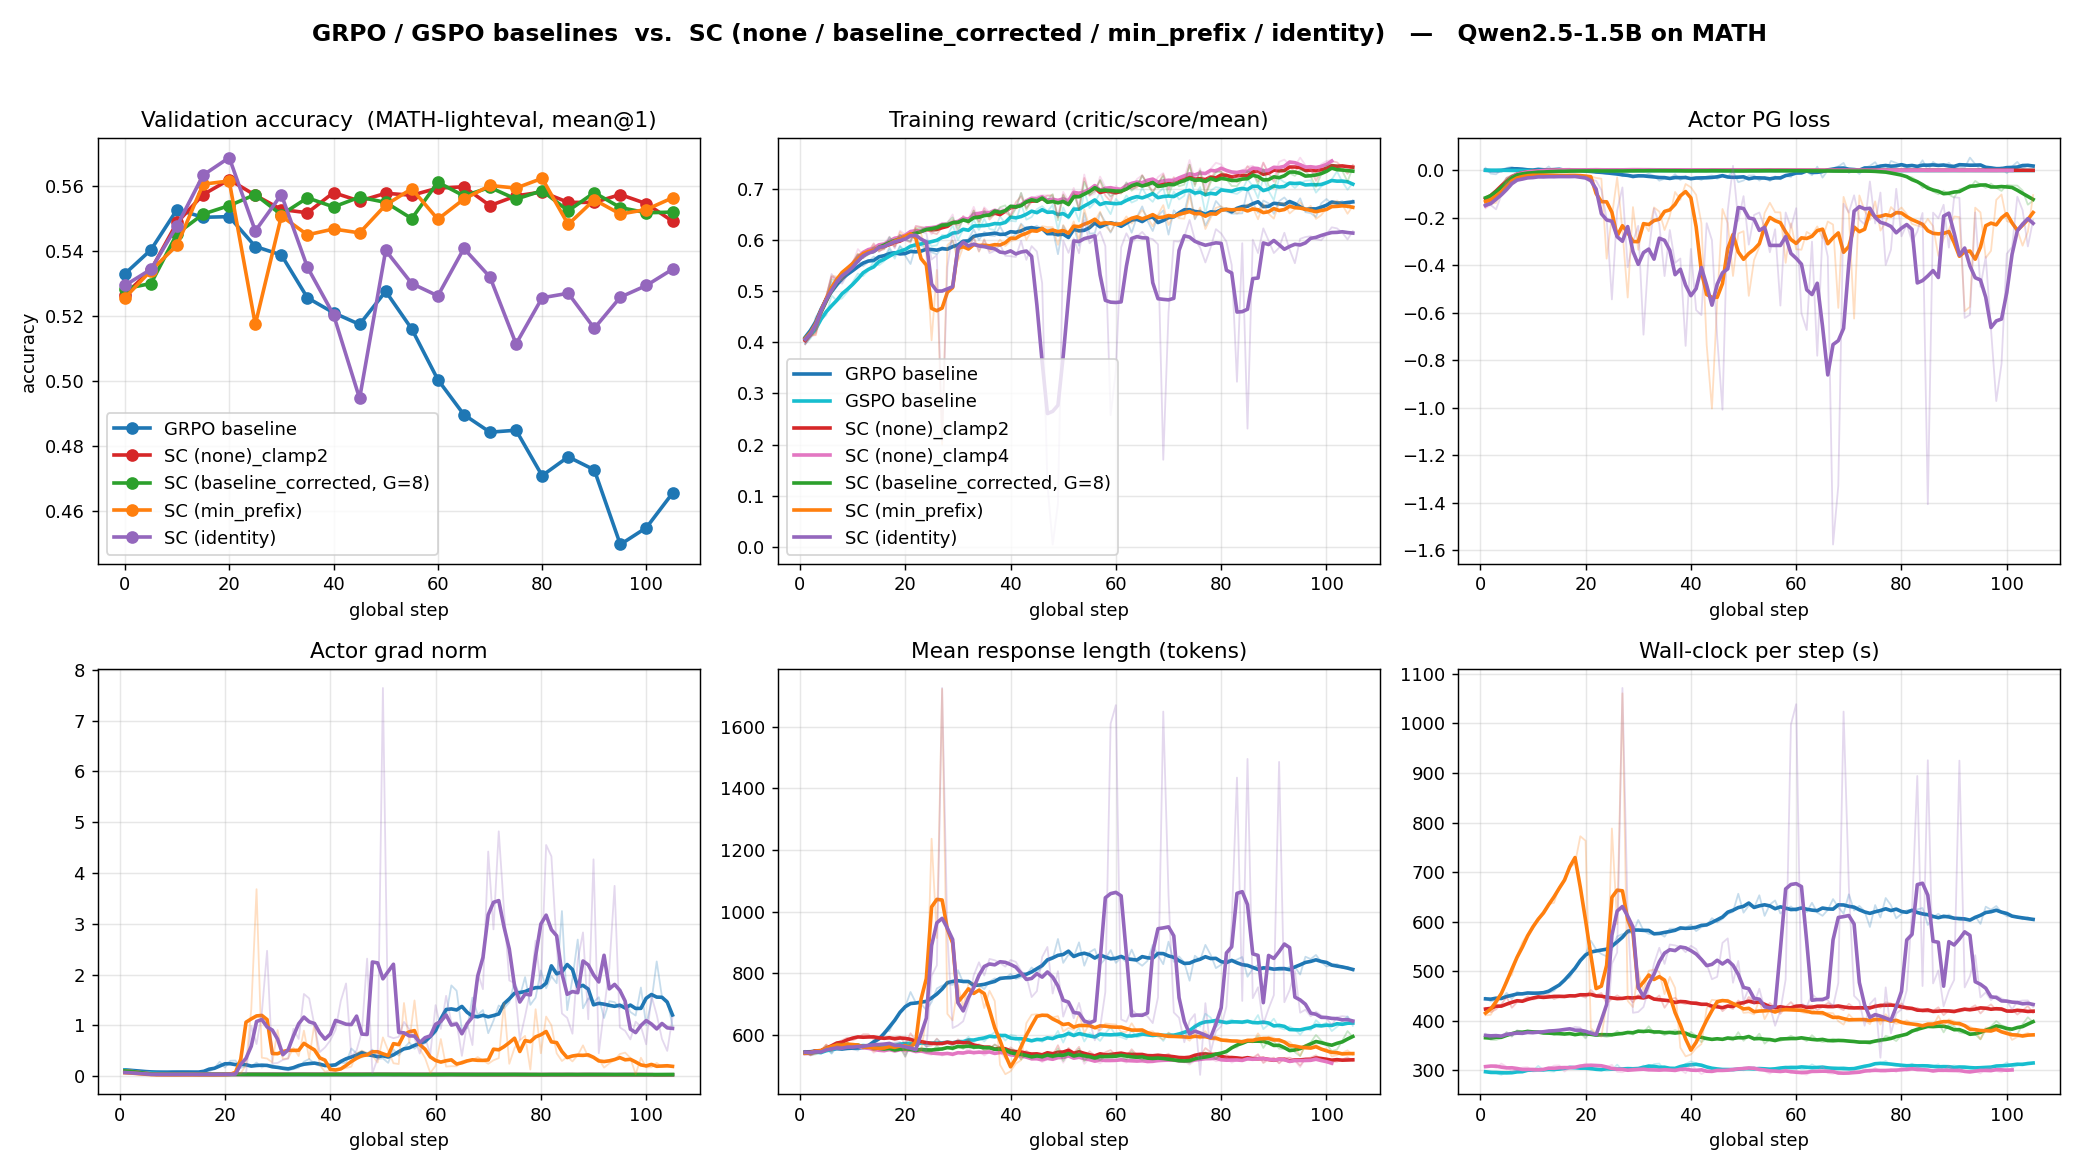
\includegraphics[width=0.95\textwidth]{../../results/comparison.png}
\caption*{Main comparison}
\end{figure}


\emph{Figure 1 --- Val-acc, training reward, PG loss, grad norm, response length, wall-clock per step.}

\begin{itemize}[leftmargin=1.2em]
\item \textbf{Val-acc (TL).} GRPO peaks at step 10 and declines steadily. \texttt{baseline\_corrected} / \texttt{min\_prefix} plateau near 0.55 and trend upward late.
\item \textbf{Train reward (TM).} \texttt{baseline\_corrected} and \texttt{none} climb fastest and highest. GRPO's train-vs-val divergence is exactly the failure mode SC targets.
\item \textbf{Response length (BM).} GRPO inflates to \textasciitilde{}770 tokens (+41 \%); \texttt{baseline\_corrected} and \texttt{none} stay at \textasciitilde{}550. Not explicitly rewarded --- a side-effect of prefix-wide pressure on every token.
\item \textbf{Wall-clock (BR).} \texttt{baseline\_corrected} fastest; CV is a single cumsum + group-mean subtract per batch.
\end{itemize}

\subsection*{5.3 What the unified trust region does}


\begin{figure}[H]
\centering
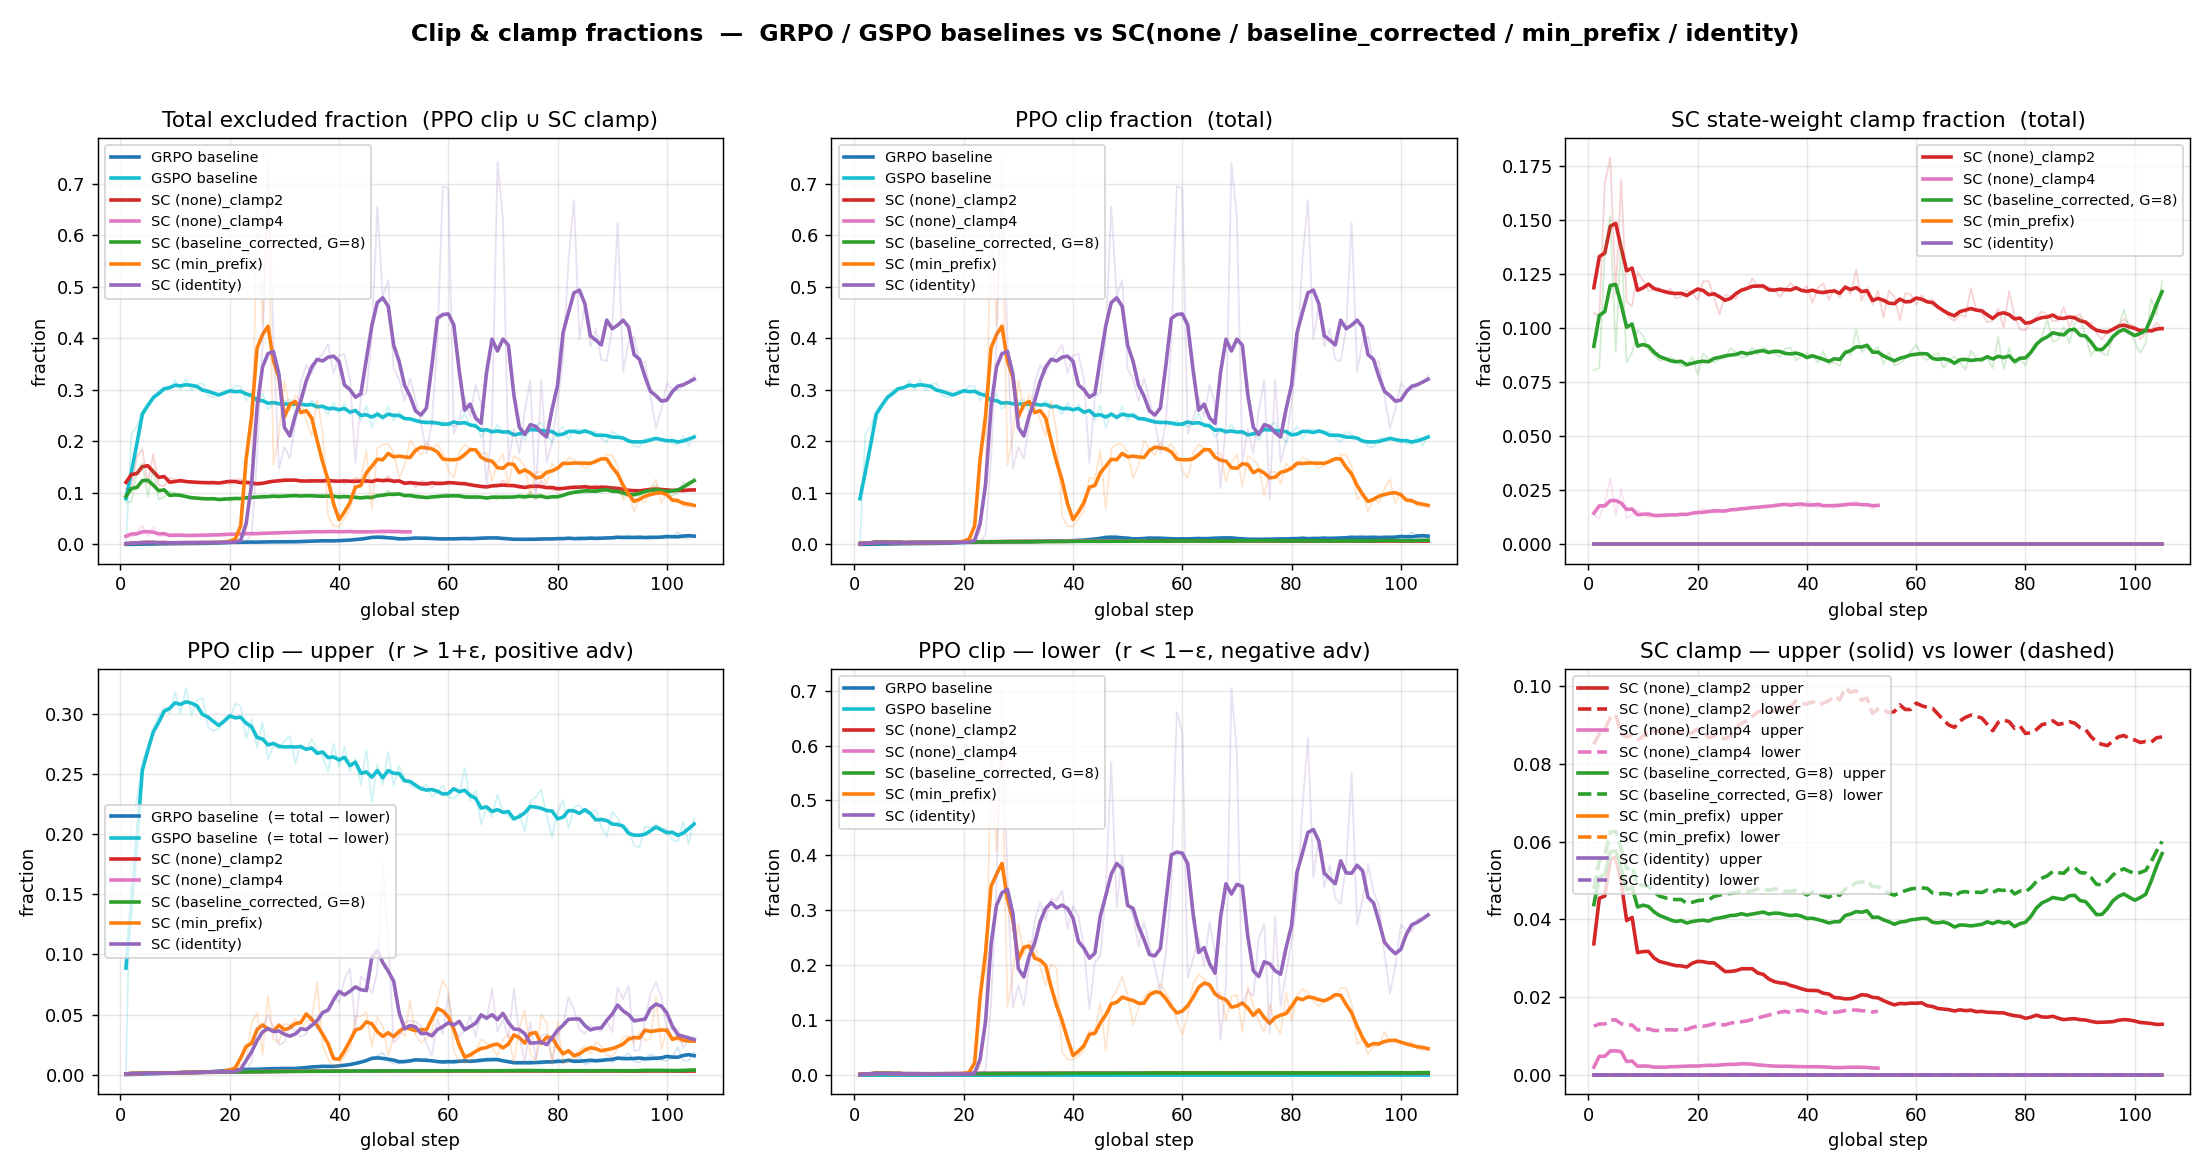
\includegraphics[width=0.95\textwidth]{../../results/comparison_clip_clamp.png}
\caption*{Clip/clamp decomposition}
\end{figure}


\emph{Figure 2 --- Top: total excluded, PPO-clip, SC-clamp. Bottom: upper/lower decomposition.}

\begin{table}[H]\centering\small
\begin{tabularx}{\textwidth}{LLLL}
\toprule
\textbf{Run} & \textbf{PPO-clip} & \textbf{SC-clamp} & \textbf{Total excluded} \\
\midrule
GRPO baseline & 0.009 & --- & 0.009 \\
SC (none) & 0.006 & 0.113 & 0.118 \\
\textbf{SC (baseline\_corrected)} & \textbf{0.006} & \textbf{0.091} & \textbf{0.097} \\
SC (min\_prefix) & 0.131 & 0.000 & 0.131 \\
SC (identity) & 0.262 & 0.000 & 0.262 \\
\bottomrule
\end{tabularx}
\end{table}

\begin{enumerate}[leftmargin=1.2em]
\item \textbf{GRPO clips almost nothing (0.9 \%).} With $|\mathcal A|\sim 10^5$, a per-token clip at one sampled action constrains \textasciitilde{}$10^{-5}$ of the simplex --- not a meaningful $D_{TV}$ proxy. A 0.9 \% clip rate coexisting with a 20-pp val-acc collapse is consistent with this.
\item \textbf{\texttt{baseline\_corrected} has the lowest total exclusion among SC runs (9.7 \%).} Drift correction pulls $\log w_t$ tightly around zero; the clamp fires less.
\item \textbf{\texttt{min\_prefix} / \texttt{identity} fail the gate differently.} SC-clamp stays at 0 (their $w_t$ rarely escapes the band) but PPO-clip balloons to 13--26 \%. Instability shows up \emph{somewhere}; Plan A just moves it to the correct gate.
\item \textbf{\texttt{baseline\_corrected}'s clamp is symmetric} (lower 4.9 \%, upper 4.2 \%); \texttt{none} is lower-heavy (9.1 \% vs 2.2 \%), reflecting the untreated Jensen drift.
\end{enumerate}

\subsection*{5.4 In one sentence}

The cross-group geometric-mean CV makes the state-ratio correction \textbf{cheap, stable, symmetric}, while \textbf{raising train reward, preserving val-acc, and cutting step time by 36 \%} versus GRPO.

\vspace{0.5em}\hrule\vspace{0.5em}
\section*{6 $\cdot$ Discussion}

\subsection*{6.1 Why \texttt{none} is competitive}

Two reasons: (i) the outer $[0.5, 2.0]$ clamp acts as an implicit V-trace --- 11.3 \% of tokens are clamped, effectively truncating the prefix product; (ii) 1.5B $\times$ 105 steps $\times$ $\leq$4096 tokens is a \emph{mild} off-policy regime. We expect the CV's advantage to grow with length and off-policy lag.

\subsection*{6.2 \texttt{SC(identity)} $\neq$ "GRPO minus state correction"}

The only methodological difference between the GRPO baseline and SC(identity) is the source of \texttt{old\_log\_prob}:

\begin{itemize}[leftmargin=1.2em]
\item \textbf{GRPO baseline} recomputes \texttt{old\_log\_prob} via a fresh actor forward pass at training precision. At step 1, $\pi_\theta=\pi_{\text{old}}$ exactly, so $r_t\equiv 1$ for every token and no token is clipped.
\item \textbf{SC(identity)} reads \texttt{old\_log\_prob} directly from the vllm rollout engine (bypass mode). Vllm runs in lower precision with a different attention kernel, so its log-probs disagree with the actor's recomputed log-probs by a small but non-zero amount --- the \textbf{training-inference mismatch}. Consequently $r_t\ne 1$ on the very first step, and a measurable fraction of tokens fall outside $[1-\epsilon,1+\epsilon]$.
\end{itemize}

This is why SC(identity) logs \texttt{actor/ppo\_clip\_frac} averaging 26 \% while the GRPO baseline stays under 2 \% --- \textbf{not because $w\equiv 1$ is unstable}, but because the vllm-vs-actor reference disagrees slightly and the clip gate catches that disagreement. The loss form itself is the same: SC(identity) and GRPO produce numerically identical gradients on in-band tokens (via $\nabla r_t = r_t\nabla\log\pi_\theta$).

Two implications:

\begin{itemize}[leftmargin=1.2em]
\item \textbf{The clean comparison is among the four SC runs}, which all share the bypass-mode \texttt{old\_log\_prob}, so \texttt{ppo\_clip\_frac} is governed only by how each $w_{i,t}$ choice interacts with the same reference. On that apples-to-apples comparison, \texttt{baseline\_corrected} has the highest training reward, the lowest total exclusion, and the most stable \texttt{joint\_active\_frac} --- attributable purely to $w_{i,t}$.
\item \textbf{The GRPO-vs-SC macro comparison} (val-acc, response length, total wall-clock) is still meaningful, but the precise clip-fraction gap between GRPO baseline and SC(identity) should not be read as "removing the state correction causes instability"; it's the reference-precision gap.
\end{itemize}

\subsection*{6.3 Exploration preservation: from \texttt{pg\_loss} $\approx$ 0 to entropy stability}

\texttt{baseline\_corrected}'s training reward climbs fastest (§6.5) while simultaneously logging a near-zero \texttt{pg\_loss}. This is \textbf{not} a contradiction --- it is the data signature of a particular structural property that we unpack here in one chain: \emph{small pg\_loss} $\leftrightarrow$ \emph{update decoupled from advantage} $\leftrightarrow$ \emph{exploration preserved} $\leftrightarrow$ \emph{faster convergence and stable entropy}.

\textbf{Step 1 $\cdot$ What small \texttt{pg\_loss} means structurally.} At fixed $t$, the SC loss (dropping constants) is


\begin{equation*}
\mathbb E[\text{pg\_loss}] \;=\; -\mathbb E_i\!\left[w_{i,t}\,r_{i,t}\,\hat A_{i,t}\,\log\pi_\theta(o_{i,t})\right].
\end{equation*}


GRPO-advantage normalisation forces $\sum_i\hat A_{i,t}=0$ within each group, so the constant-offset part cancels automatically and only a covariance survives:


\begin{equation*}
\mathbb E[\text{pg\_loss}] \;\propto\; \operatorname{Cov}_i\!\Big(\,w_{i,t}\,r_{i,t}\,\log\pi_\theta(o_{i,t}),\ \hat A_{i,t}\,\Big).
\end{equation*}


So $|\text{pg\_loss}|\approx 0$ says exactly one thing: \textbf{within each group, the quantity $w\!\cdot\! r\!\cdot\!\log\pi_\theta$ is near-independent of the rollout's advantage}. Good rollouts (large $\hat A$) and bad rollouts (small $\hat A$) are statistically indistinguishable along that axis.

\textbf{Step 2 $\cdot$ Why independence preserves exploration.} Independence means the update \emph{direction} is not forced into alignment with $\hat A$ by any confounder. Three consequences:

\begin{enumerate}[leftmargin=1.2em]
\item The policy does not collapse into a small high-reward region just to shrink $\hat A$'s variance --- it keeps its spread across rollouts.
\item The tokens the model was uncertain about keep getting visited; there's no self-reinforcing loop that concentrates probability mass into a few reward-hacking paths.
\item Per-step gradient SNR stays high, so each update is informative. \textbf{This is the mechanism behind \texttt{baseline\_corrected}'s \textasciitilde{}4$\times$ sample-complexity advantage in §6.5.}
\end{enumerate}

The gradient itself is still healthy --- \texttt{grad\_norm} is $O(10^{-1}\sim 10^0)$ across all five runs. Small \texttt{pg\_loss} is not weak training; it is the CV actively decoupling the logged scalar from the group-constant advantage offset.

\textbf{Step 3 $\cdot$ Numerical evidence.} Median $|\text{pg\_loss}|$, \texttt{grad\_norm}, and three exploration proxies:

\begin{table}[H]\centering\scriptsize
\setlength{\tabcolsep}{4pt}
\resizebox{\textwidth}{!}{%
\begin{tabular}{@{}llllll@{}}
\toprule
\textbf{Run} & \textbf{median abs pg\_loss} & \textbf{mean grad\_norm} & \textbf{mean \texttt{ppo\_clip\_frac}} & \textbf{response\_length (first $\rightarrow$ last)} & \textbf{\texttt{actor/entropy} (first/last/max)} \\
\midrule
GRPO baseline & 0.016 & 0.81 & 0.009 & 545 $\rightarrow$ \textbf{808} & 0.42 / 2.78 / \textbf{3.32} \\
SC (identity) & 0.222 & 1.15 & \textbf{0.262} & 548 $\rightarrow$ 635 & --- (not logged) \\
SC (min\_prefix) & 0.194 & 0.38 & 0.131 & 542 $\rightarrow$ 534 & --- \\
SC (none) & 0.001 & 0.035 & 0.006 & 545 $\rightarrow$ 516 & --- \\
\textbf{SC (baseline\_corrected)} & \textbf{0.003} & \textbf{0.038} & \textbf{0.006} & \textbf{545 $\rightarrow$ 593} & --- \\
\bottomrule
\end{tabular}%
}
\end{table}

Reading across the table:

\begin{itemize}[leftmargin=1.2em]
\item \textbf{GRPO baseline}: low \texttt{pg\_loss} by passive cancellation ($w=1$ is group-constant), but \textbf{no active mechanism to stop entropy from running away}. Entropy blows up 7$\times$, response length inflates 48 \%, val-acc collapses (§5.1). The independence condition holds \emph{momentarily} at the group level but not \emph{dynamically} over training.
\item \textbf{SC (identity) and SC (min\_prefix)}: large \texttt{pg\_loss} (0.19--0.22) is the direct structural evidence that $w$ is correlated with $\hat A$ --- \texttt{identity} via the bypass-mode perturbation, \texttt{min\_prefix} because small $\min r$ tracks bad rollouts. The correlation shows up macroscopically as large \texttt{ppo\_clip\_frac} (13 \% and 26 \%) and, for \texttt{identity}, response-length inflation.
\item \textbf{SC (none)} and \textbf{SC (baseline\_corrected)}: both drive the covariance to near zero, but by different routes. \texttt{none} achieves it \emph{passively} --- the raw prefix product has no structural $\hat A$-coupling. \texttt{baseline\_corrected} achieves it \emph{actively} --- cross-group centering explicitly removes any residual coupling. Both show \textbf{stable response length (\textasciitilde{}550), stable \texttt{ppo\_clip\_frac} (\textasciitilde{}0.6 \%), and preserved val-acc} --- the macroscopic fingerprint of preserved exploration.
\end{itemize}

\textbf{Step 4 $\cdot$ The feedback-loop mechanism, in concrete steps.} Why does preserving the advantage--policy independence from Step 1 actually damp entropy in practice? Three concrete gradient-dynamics arguments --- one per method --- that together explain why only \texttt{baseline\_corrected} reaches a stable exploration regime.

\emph{(a) GRPO: uncontained positive feedback on uncertainty.} Under GRPO ($w=1$), the per-token gradient contribution is $r_{i,t}\hat A_{i,t}\nabla\log\pi_\theta$. Consider a "slightly uncertain" token that happens to sit in a high-advantage rollout. After the update its probability rises, so at the next iteration $r_{i,t}>1$ for this token. The gradient weight is now larger than last step; the update pushes the probability up \emph{more aggressively}; the next $r_{i,t}$ grows further; and so on. This is a classical positive-feedback loop: \textbf{uncertainty is rewarded with amplification}, because nothing in the loss references \emph{how much the upstream prefix has already drifted}. The result is entropy runaway --- the policy keeps spreading probability onto whichever tokens happened to correlate with reward, until the distribution is flat enough that entropy hits its ceiling.

\emph{(b) SC \texttt{none}: the raw prefix corrects per-rollout drift, but not collective drift.} With $w_{i,t} = \rho_{i,1:t-1} = \prod_{j<t} r_{i,j}$, the feedback mechanism is now \textbf{second-order}: when a token's prefix drifts, its downstream $\rho$ shrinks, the gradient weight shrinks, and further amplification is damped. Per-rollout this works --- which is why \texttt{none} already gets small pg\_loss and stable response length. But $\rho_{i,1:t-1}$ still has a \emph{collective} failure mode: if the entire group drifts in the same direction (e.g. everyone's early-position probability shifts), then $\mathbb E[\log\rho_{1:t-1}]\approx -(t-1)\bar D_{\mathrm{KL}}$ keeps growing --- every rollout's weight shrinks by the same factor. The outer clamp $[w_{\min}, w_{\max}]$ catches the tails, but at the cost of silently dropping \textasciitilde{}11 \% of tokens from the gradient (§5.3). The mechanism works, but leaves residual bias that the clamp has to mop up.

\emph{(c) SC \texttt{baseline\_corrected}: the CV removes the collective-drift mode.} The weight is
\[
w_{i,t} \;=\; \rho_{i,1:t-1}\big/\mathrm{GM}_{\mathrm{grp}(i)}\,\rho_{1:t-1}
\qquad(\mathrm{GM}=\text{GeoMean}),
\]
i.e.\ a \textbf{ratio of absolute drifts within the group}. If the whole group drifts together, the numerator and denominator both shrink by the same factor and $w_{i,t}$ stays near $1$. What the gradient weight sees is \textbf{only the relative drift of this rollout vs its group peers}, not the absolute drift of the group as a whole. Concretely this changes the feedback dynamics in three ways:

\begin{enumerate}[leftmargin=1.2em]
\item \textbf{No collective amplification.} The GRPO failure mode --- all rollouts in a group sliding uncertainty upward together --- is invisible to $w$, so it cannot feed back into amplification.
\item \textbf{Within-group contrast is preserved.} A rollout whose prefix drifted \emph{more} than its peers (bad rollout) gets $w<1$, damping its gradient; a rollout that stayed closer to $\pi_\beta$ than its peers (good rollout) gets $w>1$, amplifying its gradient. This is exactly what we want --- the CV is a per-position "credit assignment" that says \emph{which rollout in this group should teach the policy the most}.
\item \textbf{Clamp has less to do.} Because the group mean is subtracted first, only genuine \emph{within-group outliers} need to be clamped; the clamp fraction drops from 11 \% (\texttt{none}) to 9.7 \% (\texttt{baseline\_corrected}, §5.3), and is symmetric (upper $\approx$ lower $\approx$ 4 \%).
\end{enumerate}

Put together: under GRPO, uncertainty amplifies itself; under \texttt{none}, per-rollout amplification is damped but collective amplification is not; under \texttt{baseline\_corrected}, \textbf{both are damped}, because the weight only responds to relative --- never absolute --- drift. The independence condition from Step 1 is not an accident: it is the algebraic statement of "the state weight has been made blind to group-wide drift", which is \emph{exactly} the property that closes the entropy-runaway loop.

This also explains the empirical table: \texttt{none} and \texttt{baseline\_corrected} sit in the same exploration-preserving regime on all four proxies (pg\_loss $\approx$ 0, stable grad\_norm, stable clip\_frac, stable length), while GRPO and \texttt{identity} blow up entropy via (a), and \texttt{min\_prefix} sits in between because $\min_{j<t} r_j$ captures worst-case but not average prefix drift --- partial damping without the group-centering that would close the loop.

So across runs: \textbf{\texttt{pg\_loss} near zero + stable \texttt{grad\_norm} + stable \texttt{ppo\_clip\_frac} + stable response length} is a four-way coherent signature of the exploration-preserving regime. \texttt{baseline\_corrected} is the only method that reaches this regime structurally (via the CV) rather than by accident --- which is why its training reward (and val-acc) keeps climbing where GRPO's collapses.

\subsection*{6.4 Convergence speed}

Two factors: steps-to-target $\times$ time-per-step.

\textbf{Steps-to-target} (first step at train reward $\geq$ 0.68, reading smoothed Figure 1):

\begin{table}[H]\centering\small
\begin{tabularx}{\textwidth}{LL}
\toprule
\textbf{Run} & \textbf{First step $\geq$ 0.68} \\
\midrule
GRPO baseline & \textasciitilde{}95 \\
SC (none) & \textasciitilde{}25 \\
\textbf{SC (baseline\_corrected)} & \textbf{\textasciitilde{}25} \\
SC (min\_prefix) & \textasciitilde{}80 \\
SC (identity) & never \\
\bottomrule
\end{tabularx}
\end{table}

\texttt{baseline\_corrected} is \textasciitilde{}4$\times$ faster in sample-complexity. The mechanism is that group-mean-centered advantage gives $\nabla L\propto \text{Cov}_{\text{group}}(w_t,\hat A_t)$; a good rollout's prefix stays close to $\pi_\theta$ ($w\approx 1$), a bad one's drifts ($w$ clamped small). \textbf{The state weight sharpens the contrast between good and bad rollouts inside a group}, amplifying gradient SNR.

\textbf{Per-step cost}: 372 s vs 580 s. Three sources: \texttt{bypass\_mode} saves one forward; Plan-A mask is one op vs. double-min; fewer active tokens in backward.

\textbf{Combined}: 25$\times$372 $\approx$ 9,300 s vs 95$\times$580 $\approx$ 55,100 s $\rightarrow$ \textbf{$\approx$ 6$\times$ total wall-clock to target}. Even discounting the noisy steps-to-target estimate, the 1.56$\times$ step-time factor alone stands.

\subsection*{6.5 What remains to test}

\begin{itemize}[leftmargin=1.2em]
\item \textbf{Larger models} (7B, 14B) and \textbf{longer sequences} --- prefix variance grows, CV should matter more.
\item \textbf{Off-policy lag} (rollouts 2+ steps behind), where GRPO/GSPO/CISPO are known to collapse.
\item \textbf{$G$ ablation} --- the CV baseline tightens as $G$ grows; $G\in\{16,32\}$ is the natural test.
\item \textbf{Combining with DPPO-style $D_{TV}$} --- state correction and action-distribution correction are orthogonal.
\end{itemize}

\vspace{0.5em}\hrule\vspace{0.5em}
\section*{7 $\cdot$ Takeaway}

The state ratio that every GRPO-family method drops is, in LLMs, \textbf{not intractable} --- it is an already-computed product of per-token log-ratios. The only real engineering question is variance.

\texttt{baseline\_corrected} answers it with a control variate: starting from the exact per-token IS form $\rho_{1:t-1}\!\cdot\! r_t$ (Theorem~\ref{thm:is-unbiased}), dividing by the cross-group geometric mean of $\rho_{1:t-1}$ leaves the on-policy limit invariant (Theorem~\ref{thm:bc-unbiased}\ref{thm:bc:onpolicy}) while exactly cancelling the linear-in-$t$ Jensen drift in log-space (Theorem~\ref{thm:bc-unbiased}\ref{thm:bc:logunbiased}). The baseline is free and group-native --- no extra forward, no extra hyper-parameter.

On Qwen2.5-1.5B / MATH / 105 steps:

\begin{itemize}[leftmargin=1.2em]
\item \textbf{+7 pp training reward} (0.741 vs 0.677)
\item \textbf{+9 pp val-acc at step 105} (0.552 vs 0.465) --- GRPO overfits, SC-BC doesn't
\item \textbf{$-$36 \% wall-clock per step}
\item \textbf{lowest total-exclusion fraction} among SC variants (9.7 \%)
\end{itemize}

No extra parameters, no extra forward passes, no extra reward shaping --- the correction the literature discarded is waiting to be added back.

\end{document}
